\section{Initial Results}
30 minutes of random load noise was applied to the system where every governor in the system had an identical deadband.
Each type of deadband shown in Fig. \ref{fig: deadbandType} was simulated.
An experiment was also conducted to explore partial acceptance of the NERC recommendations presented in \cite{nercFRI2012}.
While PSLTDSim can model AGC, it was not enabled for these simulations.


\subsection{System Modifications}
The miniWECC system was modified to include three areas for simulation.
PSLTDSim was used to set all area governor deadbands to 5\%.
Governors were removed from some units so that only $\approx$20\% of generation capacity in each area has governor control.
%A generic AGC routine that filters area control error (ACE) through a proportional-intergal (PI)  controller was added to each area.
%AGC messages are sent select generation units with governors representing $\approx$9\% of total generation capacity every 15 seconds.

\subsection{System Noise Injection}
Noise was injected into every load in the system according to
\begin{align}
P_{L} &= P_{L}(1 \pm N_Z Rand) \label{eq: noise}
\end{align}
where $N_Z$ represents the maximum amount of random noise to inject as a percent,
and $Rand$ is randomly generated for each load as a number between 0 and 1 inclusive.
The decision to add or subtract noise is chosen by another randomly generated number.
As shown, (\ref{eq: noise}) creates random walk behavior in load value as this is more representative of real life power systems\cite{AGCCresap}.


\subsection{Noise Simulation Results}
30 minutes were simulated where $N_Z$ was set to 0.03. 
The noise added system loading is shown in Fig. \ref{fig: systemLoading} while Fig. \ref{fig: sysFreqDB} shows the resulting system frequency for each type of deadband.

\begin{figure}[!ht]
\centering
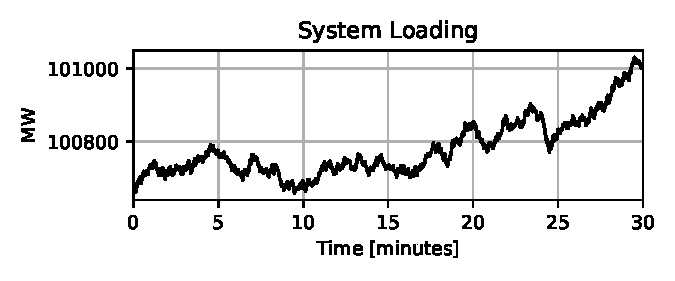
\includegraphics[width=\linewidth]{figures/miniWECCuniAccPload}
\caption{Total system loading.}
\label{fig: systemLoading}
\end{figure}

\begin{figure}[!ht]
\centering
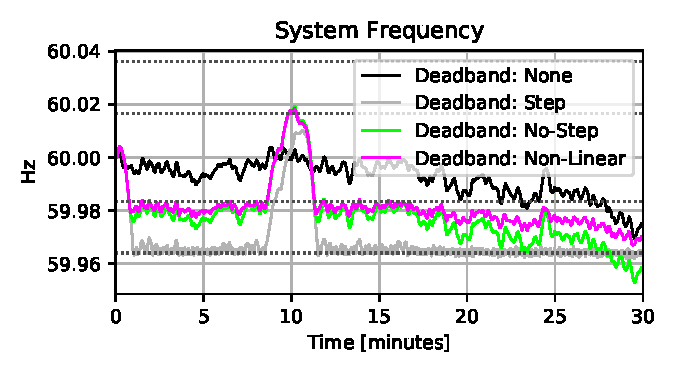
\includegraphics[width=\linewidth]{figures/miniWECCnoiseNLdroopDBFreq}
\caption{System frequency of various deadbands.}
\label{fig: sysFreqDB}
\end{figure}

As shown in Fig. \ref{fig: valveComp} a step deadband sends a step input to the governor valve when system frequency is oscillating near the deadband. These control pulses greatly increase valve travel over the more linear methods.

\begin{figure}[!ht]
\centering
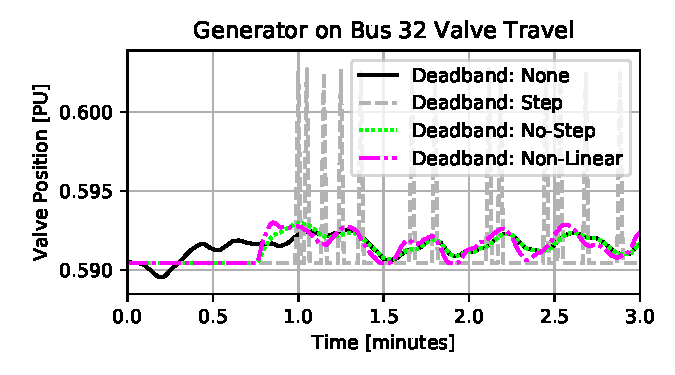
\includegraphics[width=\linewidth]{figures/gen32ValveComp}
\caption{Deadband valve movement comparisons.}
\label{fig: valveComp}
\end{figure}

Table \ref{tab: valveTravel} summarizes the valve travel for each generator in the system over the entire 30 minute simulation.

% Testing of external table build for \input later
% Uses the IEEE table format guidelines
\begin{table}[!ht]
	\caption{Total valve travel for various deadband scenarios.}
	\label{tab: valveTravel}
	\centering
	\begin{tabular}{@{} C{1cm} S[table-format=2.2] S[table-format=2.2] S[table-format=2.2] S[table-format=2.2] S[table-format=2.2] @{}} 	
							\toprule							
		&	\multicolumn{5}{c}{Valve Travel [PU]}							\\	
	\text{Generator}	&	\text{No DB}	&	\text{Step}	&	\text{No-Step}	&	\text{\shortstack{N-L\\Droop}}  &	\text{\shortstack{No-Step\\Non-H}}	\\	\midrule	
	17	&	0.16	&	7.48	&	0.15	&	0.23	& 0.19 \\	
	23	&	0.16	&	7.48	&	0.15	&	0.23	& 0.19 \\	
	30	&	0.16	&	7.48	&	0.15	&	0.23	& 0.19 \\	
	32	&	0.16	&	7.54	&	0.15	&	0.23	& 0.19 \\	
	107	&	0.16	&	7.54	&	0.15	&	0.23	& 0.19 \\	
	41	&	0.15	&	6.44	&	0.14	&	0.23	& 0.06 \\	
	45	&	0.15	&	6.44	&	0.14	&	0.23	& 0.06 \\	
	53	&	0.16	&	7.54	&	0.15	&	0.23	& 0.06 \\	
	59	&	0.15	&	6.44	&	0.14	&	0.23	& 0.06 \\	\bottomrule
	Total:	&	1.41	&	64.38	&	1.32	&	2.07& 1.19 	\\	

	\end{tabular}

\end{table}


\subsection{Universal Acceptance Simulation Results}
To test partial acceptance of NERC recommendations, all area deadbands were set to the no step variety, but two of the three areas had a deadband of 16.6 mHz while the third deadband was 36 mHz.

As expected, Fig. \ref{fig: areaValveTravel} shows that the area with a larger deadband doesn't respond while the other areas with a smaller deadband do.
\begin{figure}[!ht]
\centering
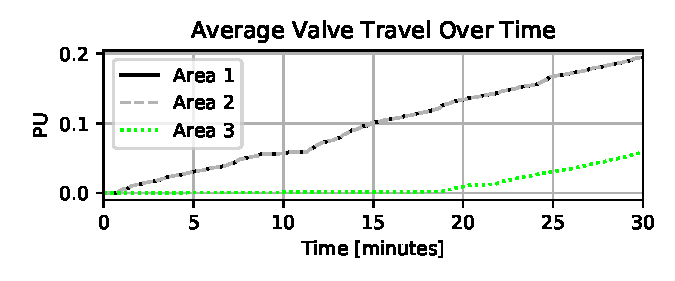
\includegraphics[width=\linewidth]{figures/miniWECCuniAccVTOverTime}
\caption{Area average valve travel.}
\label{fig: areaValveTravel}
\end{figure}